\documentclass{article}

\usepackage{neurips_2024}

\usepackage[utf8]{inputenc}
\usepackage[T1]{fontenc}
\usepackage{hyperref}
\usepackage{url}
\usepackage{booktabs}
\usepackage{multirow}
\usepackage{amsfonts}
\usepackage{nicefrac}
\usepackage{microtype}
\usepackage{amssymb}
\usepackage{amsmath}
\usepackage{graphicx}
\usepackage{subcaption}

\title{When Do Quantum Kernels Help? \\ An Empirical and Diagnostic Study of the ZZ Feature Map}

\author{
  Anonymous Author(s) \\
  Affiliation \\
  \texttt{email@domain.com}
}

\begin{document}

\maketitle

\begin{abstract}
Quantum kernel methods promise richer feature spaces than classical kernels by
encoding data into the exponentially large Hilbert space of a quantum circuit,
but it is unclear how often this promise translates into an actual advantage
on realistic data. We build a from-scratch, exactly-simulated implementation
of the Havl{\'i}\v{c}ek et al.\ (2019) ZZ feature-map fidelity kernel --
without any quantum computing library -- validate it against an independent
brute-force construction, and use it to run a controlled comparison against
classical (RBF, polynomial, linear) kernels under an identical model-selection
protocol. On a synthetic dataset engineered so its labels are a function of
the same feature map (a positive control), the quantum kernel reaches
$98.3\%$ test accuracy versus $48$--$53\%$ (chance level) for every classical
kernel. On two standard tabular UCI benchmarks (Wine, Breast Cancer) with no
such engineered structure, the result reverses sharply: classical kernels
reach $92$--$98\%$ accuracy while the quantum kernel collapses to
$66.7\%$ -- on Wine, exactly the majority-class baseline. We diagnose this
gap using kernel-target alignment and kernel-value statistics, and connect it
to existing theory on the inductive bias and concentration of quantum
kernels. Our results are an honest negative result for quantum kernels as a
drop-in replacement for classical kernels on generic data, and a clean
positive control demonstrating our simulator and evaluation protocol are
correct and can detect an advantage when one is present by construction.
\end{abstract}

\section{Introduction}

Quantum kernel methods encode a classical data point $x$ into a quantum state
$|\phi(x)\rangle$ via a parameterized circuit (a \emph{feature map}), and
define a kernel as an inner product between such states, $k(x,x') =
|\langle\phi(x)|\phi(x')\rangle|^2$. Because $|\phi(x)\rangle$ lives in a
Hilbert space of dimension $2^n$ for $n$ qubits, this is often motivated as
implicitly using an exponentially large feature space that would be
classically intractable to represent explicitly
\citep{rebentrost2014quantum, schuld2019quantum, havlicek2019supervised}.
This is the same kernel-trick argument used to motivate the RBF kernel, and
it raises an obvious empirical question: for a fixed, modest number of
qubits, does a quantum kernel actually classify real data any better than a
well-tuned classical kernel with the same number of input features?

The honest answer, as several theoretical results have begun to suggest
\citep{kubler2021inductive, huang2021power, thanasilp2024exponential}, is
usually no -- unless the data has structure specifically aligned with the
feature map. We investigate this question directly and empirically. Rather
than relying on a quantum SDK (which can obscure what the kernel is actually
computing behind a compiled circuit and a stochastic shot-based estimate), we
implement an \emph{exact}, from-scratch classical simulation of the
Havl{\'i}\v{c}ek et al.\ ZZ feature map kernel using only NumPy, and validate
it bit-for-bit against an independent brute-force dense-matrix
implementation. We then run the same model-selection and evaluation protocol
for the quantum kernel and three classical kernels (RBF, polynomial, linear)
on: (1) a synthetic dataset explicitly engineered, following
\citet{havlicek2019supervised}, so that its ground-truth labels are a
function of the same feature map -- a positive control that should favor the
quantum kernel; and (2) two standard UCI tabular datasets (Wine, Breast
Cancer) with no such engineered relationship to any quantum feature map --
datasets a practitioner might realistically want to classify.

\textbf{Contributions.}
\begin{itemize}
  \item An exact, dependency-free NumPy simulator of the ZZ feature-map
  fidelity kernel, using a batched Walsh--Hadamard transform and a vectorized
  diagonal-phase update, validated against an independent brute-force
  dense-matrix construction (Section~\ref{sec:method}).
  \item A reproduction of the Havl{\'i}\v{c}ek-style engineered
  ``quantum-advantage'' dataset construction, together with a fully
  worked-out, checkable derivation of its labeling rule
  (Section~\ref{sec:synthetic}).
  \item A controlled empirical comparison, under one shared model-selection
  protocol and a common kernel normalization, of the quantum kernel against
  classical kernels on both the engineered positive control and two real
  UCI benchmarks (Sections~\ref{sec:setup}--\ref{sec:results}).
  \item A diagnosis of \emph{why} the quantum kernel fails on real data
  using kernel-target alignment \citep{cristianini2001kernel} and raw
  kernel-value statistics, connected to the inductive-bias and
  concentration-of-measure literature (Section~\ref{sec:discussion}).
\end{itemize}

We are explicit about what this study does \emph{not} claim: because exact
classical simulation costs $O(2^n)$ per sample, we can only evaluate small
qubit counts ($n \le 6$), so nothing here bears on whether a real quantum
device would offer a \emph{computational} (runtime) advantage. Our claim is
narrower and purely statistical: for the ZZ feature map at accessible qubit
counts, whether the resulting kernel is a good inductive bias for a
classification task depends entirely on whether the task's structure matches
the feature map -- it is not a general-purpose upgrade over classical
kernels.

\section{Background and Related Work}
\label{sec:background}

\textbf{Quantum kernel methods.} \citet{rebentrost2014quantum} first proposed
a quantum algorithm for kernel-based classification with an asymptotic
speedup under strong data-access assumptions. \citet{schuld2019quantum} and
\citet{havlicek2019supervised} reformulated quantum classifiers as kernel
methods operating in a feature Hilbert space defined by a data-encoding
circuit, making the standard kernel-trick machinery (e.g., support vector
machines \citep{cortes1995support}) directly applicable once the kernel
matrix is computed -- either by a quantum device or, at small scale, by
classical simulation, as we do here. \citet{havlicek2019supervised} also
introduced the specific ZZ feature map we use, along with a synthetic dataset
construction, discussed in Section~\ref{sec:synthetic}, designed to have a
large margin in the induced feature space and thus be provably easy for the
associated kernel.

\textbf{When quantum kernels do (not) help.} A growing body of theoretical
work argues that quantum kernels are not a universal upgrade.
\citet{huang2021power} show that without structure in the data or in the
choice of feature map, quantum models offer no advantage over classical ones
and can be matched by classical kernels informed by the same data.
\citet{kubler2021inductive} formalize this as an inductive-bias question: a
generic quantum feature map induces a kernel whose implied prior over
functions is often a poor match for real learning tasks, leading to worse
generalization than a well-chosen classical kernel unless the feature map is
tailored to the problem. \citet{thanasilp2024exponential} show that for many
families of quantum kernels, off-diagonal kernel values concentrate
exponentially closely (in the number of qubits) around a fixed value as
problem size grows, which drives the Gram matrix toward a constant matrix and
the resulting classifier toward predicting the majority class -- exactly the
failure mode we observe empirically in Section~\ref{sec:results}. Our
contribution relative to this literature is not new theory but a careful,
reproducible, fully-classical empirical demonstration: the same simulator,
normalization, and model-selection protocol applied to both an engineered
positive control and unmodified real tabular data, with the resulting gap
diagnosed rather than merely reported.

\textbf{Kernel-target alignment.} \citet{cristianini2001kernel} propose
kernel-target alignment as a measure of how well a kernel's geometry matches
a labeling function, independent of any specific classifier. We use it as a
label-aware diagnostic to complement the label-agnostic kernel-value
statistics of \citet{thanasilp2024exponential}.

\section{Method}
\label{sec:method}

\subsection{The ZZ feature map and fidelity kernel}

For $n$ qubits and input $x \in \mathbb{R}^n$, the ZZ feature map applies
$R$ repetitions of a layer consisting of a Hadamard transform followed by a
diagonal unitary encoding $x$:
\[
U_\phi(x) = \left[ \exp\!\Big(i \sum_{j} x_j Z_j + i\!\!\sum_{j<k}\!(\pi -
x_j)(\pi - x_k)\, Z_j Z_k\Big)\, H^{\otimes n} \right]^{R},
\qquad |\phi(x)\rangle = U_\phi(x)\,|0\rangle^{\otimes n},
\]
where $Z_j$ is the Pauli-$Z$ operator on qubit $j$. This is the ``full
entanglement'' variant of \citet{havlicek2019supervised}: every pair of
qubits is coupled through the $(\pi - x_j)(\pi - x_k)$ term. We use $R=2$
throughout. The fidelity kernel is
$k(x, x') = |\langle \phi(x) | \phi(x') \rangle|^2 \in [0, 1]$.

\subsection{Exact simulation without a quantum SDK}

Because the encoding unitary is diagonal in the computational basis, the
circuit reduces to alternating (i) a Walsh--Hadamard transform and (ii) an
elementwise complex phase multiply -- no gate-by-gate simulation or quantum
library is required. Writing $s_i(z) = (-1)^{z_i}$ for the $i$-th bit of
basis state $z$, the phase applied to $|z\rangle$ is
\[
\theta(z, x) = \sum_i x_i\, s_i(z) \;+\; \sum_{i<j} (\pi - x_i)(\pi -
x_j)\, s_i(z) s_j(z).
\]
Using $s_i(z)^2 = 1$, the pairwise sum can be rewritten in closed form as
$\tfrac{1}{2}\big[(\sum_i u_i s_i(z))^2 - \sum_i u_i^2\big]$ with $u = \pi -
x$, which lets us compute $\theta(\cdot, x)$ for all $2^n$ basis states and a
batch of $N$ samples with two matrix multiplications instead of an
$O(n^2)$ loop over qubit pairs. The batched Walsh--Hadamard transform is
applied by reshaping the $N \times 2^n$ state array to $N \times
\underbrace{2 \times \cdots \times 2}_{n}$ and butterflying each axis, giving
$O(N n 2^n)$ total cost per repetition -- exact, and, for the $n \le 6$
qubits used in this paper, fast enough to run all experiments in under two
seconds on a laptop CPU.

\textbf{Correctness.} We validate this vectorized implementation against an
independent brute-force construction that builds the dense $2^n \times 2^n$
Hadamard matrix via Kronecker products and the diagonal phase matrix via an
explicit double loop over qubit pairs, for $n \in \{1,2,3,4\}$ and $R \in
\{1,2,3\}$ with random inputs. The two implementations agree to within
$10^{-10}$ in every case. We additionally check, over $50$ random $5$-qubit
inputs, that every simulated state has unit norm (confirming the circuit is
unitary), and that resulting kernel matrices are symmetric, have unit
diagonal, and are positive semi-definite (minimum eigenvalue $> -10^{-8}$),
as required of a valid Gram matrix.

\subsection{Kernel normalization}

Classical kernel values are not restricted to $[0,1]$: on our data (features
scaled to $[0, 2\pi)$, Section~\ref{sec:setup}), an unnormalized degree-3
polynomial kernel can reach entries of order $10^4$--$10^5$. In preliminary
runs this made libsvm's QP solver (default \texttt{max\_iter}$=-1$, i.e.\
unbounded) take pathologically long to converge on the polynomial kernel,
effectively hanging the benchmark. We fix this, and simultaneously put all
kernels on a comparable footing for the alignment analysis, by normalizing
every Gram matrix to unit diagonal, $\hat k(x,x') = k(x,x') /
\sqrt{k(x,x)\,k(x',x')}$, before model fitting. This is a no-op for the
quantum kernel, which already satisfies $k(x,x)=1$ by construction. As a
safety net we also cap the SVM solver at $2\times10^5$ iterations for every
kernel.

\subsection{Kernel-target alignment}

Following \citet{cristianini2001kernel}, for labels $y \in \{-1,+1\}^N$ and
Gram matrix $K$ we report
\[
A(K, y) = \frac{\langle K,\, yy^\top \rangle_F}{\lVert K \rVert_F\,
\lVert yy^\top \rVert_F},
\]
a label-aware measure, in $[-1,1]$, of how well the kernel's similarity
structure matches the target labeling, independent of any specific
downstream classifier.

\subsection{Synthetic quantum-advantage dataset}
\label{sec:synthetic}

We reproduce the engineered positive-control construction of
\citet{havlicek2019supervised}. Fix a Haar-random $2^n \times 2^n$ unitary
$V$ (sampled via QR decomposition of a complex Gaussian matrix with the
phase correction of \citet{mezzadri2007generate}) and a fixed non-trivial
Pauli-$Z$-string observable $P = \mathrm{diag}(f)$, $f_z = (-1)^{\mathrm{parity}(z
\,\&\, \mathrm{mask})}$ for a random non-zero bitmask. Define the rotated
observable $M = V P V^\dagger$ and, for a candidate point $x$, its margin
under the feature map,
\[
m(x) = \langle \phi(x) | M | \phi(x) \rangle
     = \sum_z \big|\langle z | V^\dagger | \phi(x) \rangle\big|^2\, f_z ,
\qquad y(x) = \mathrm{sign}\big(m(x)\big).
\]
We draw $x$ uniformly from $[0, 2\pi)^n$ and keep only points with $|m(x)|
\ge \gamma$, discarding the rest; this yields, by construction, a dataset
that is separable by the quantum kernel with margin at least $\gamma$ in the
$V$-rotated feature space, while making no promise about the existence of an
easy classical decision boundary. We build two such datasets: $n=4$ qubits,
$\gamma=0.3$, and a harder, higher-dimensional $n=6$ qubits, $\gamma=0.2$,
each with $200$ class-balanced samples.

\section{Experimental Setup}
\label{sec:setup}

\textbf{Datasets.} In addition to the two synthetic datasets above, we use
two standard UCI classification benchmarks via scikit-learn
\citep{pedregosa2011scikit}: \emph{Wine} (one class vs.\ rest, $178$
samples) and \emph{Breast Cancer Wisconsin} (malignant vs.\ benign, $569$
samples). For both, we standardize features, project to $4$ principal
components (matching $n=4$ qubits) with PCA, and rescale to $[0, 2\pi)$ with
a min-max scaler -- the same representation is fed to every kernel, so
comparisons isolate the choice of kernel rather than confounding it with
different preprocessing.

\textbf{Baselines.} RBF, polynomial (degree $\in \{2,3\}$, $\mathrm{coef0}=1$),
and linear kernels, via scikit-learn's pairwise-kernel functions, each fed
into an SVM with a precomputed Gram matrix.

\textbf{Model selection.} For every (dataset, kernel-family) pair we sweep a
hyperparameter grid (RBF: $\gamma \in \{0.02, 0.05, 0.1, 0.2, 0.5\}$;
polynomial: degree $\in \{2,3\}$; quantum and linear: no kernel
hyperparameter beyond the fixed construction above) and, for each setting,
select the SVM regularization constant $C \in \{0.1, 1, 3, 10, 30, 100\}$ by
$5$-fold stratified cross-validation on a $70\%$ training split, then report
accuracy on the untouched $30\%$ test split, refitting once on the full
training split with the selected hyperparameters. This identical protocol is
applied to all four kernel families. All experiments use seed $0$ for the
train/test split and the CV folds.

\textbf{Implementation.} All kernels, the SVM wrapper, and the model
selection loop are implemented once and shared across kernel families
(Section~\ref{sec:method}), so no part of the pipeline is quantum-specific
except the kernel matrix computation itself.

\section{Results}
\label{sec:results}

\begin{table}[t]
  \caption{Test accuracy, cross-validation accuracy, and kernel-target
  alignment for the best hyperparameter setting of each kernel family
  (selected by CV accuracy), on each dataset. Bold marks the best test
  accuracy per dataset. Majority-class baselines: $50.0\%$ (both synthetic
  datasets, class-balanced by construction), $66.7\%$ (Wine), $62.6\%$
  (Breast Cancer).}
  \label{tab:main}
  \centering
  \small
  \begin{tabular}{llccc}
    \toprule
    Dataset & Kernel & CV acc.\ & Test acc.\ & Alignment \\
    \midrule
    \multirow{4}{*}{Synthetic ($n{=}4$, $\gamma{=}0.3$)}
      & Quantum (ZZ) & $1.000$ & $\mathbf{0.983}$ & $0.166$ \\
      & RBF          & $0.657$ & $0.483$ & $0.084$ \\
      & Polynomial   & $0.593$ & $0.483$ & $0.002$ \\
      & Linear       & $0.500$ & $0.483$ & $0.001$ \\
    \midrule
    \multirow{4}{*}{Synthetic ($n{=}6$, $\gamma{=}0.2$)}
      & Quantum (ZZ) & $0.843$ & $\mathbf{0.733}$ & $0.095$ \\
      & RBF          & $0.614$ & $0.467$ & $0.062$ \\
      & Polynomial   & $0.643$ & $0.450$ & $0.014$ \\
      & Linear       & $0.607$ & $0.533$ & $0.005$ \\
    \midrule
    \multirow{4}{*}{Wine (PCA-4)}
      & Quantum (ZZ) & $0.669$ & $0.667$ & $0.108$ \\
      & RBF          & $0.984$ & $0.944$ & $0.236$ \\
      & Polynomial   & $0.976$ & $\mathbf{0.981}$ & $0.142$ \\
      & Linear       & $0.935$ & $0.926$ & $0.121$ \\
    \midrule
    \multirow{4}{*}{Breast Cancer (PCA-4)}
      & Quantum (ZZ) & $0.718$ & $0.667$ & $0.073$ \\
      & RBF          & $0.982$ & $\mathbf{0.936}$ & $0.286$ \\
      & Polynomial   & $0.980$ & $0.942$ & $0.130$ \\
      & Linear       & $0.962$ & $0.947$ & $0.101$ \\
    \bottomrule
  \end{tabular}
\end{table}

Table~\ref{tab:main} shows the central result. On both engineered datasets,
the quantum kernel dominates every classical kernel by a wide margin
($98.3\%$ vs.\ $\le 48.3\%$ at $n{=}4$; $73.3\%$ vs.\ $\le 53.3\%$ at
$n{=}6$, with all classical kernels within a few points of the $50\%$
chance level). On the two real datasets, the ranking reverses completely:
classical kernels reach $92$--$98\%$ test accuracy while the quantum kernel
falls to $66.7\%$ on both -- on Wine, this is \emph{exactly} the
majority-class baseline, and on Breast Cancer it is only $4.1$ points above
it, versus $27$--$32$ points above baseline for every classical kernel.

\textbf{Sample efficiency.} Figure~\ref{fig:learning-curves} tracks test
accuracy as a function of training set size. On the engineered dataset
(left), the quantum kernel improves steadily from $72\%$ at $10$ training
points to $96\%$ at $130$, while every classical kernel is flat at
chance level regardless of how much data it sees -- more data does not help
a kernel whose inductive bias does not match the task. On Wine (right), the
pattern is a mirror image: all three classical kernels climb quickly to
$92$--$98\%$, while the quantum kernel is a flat line at $66.7\%$ from the
smallest training size onward, i.e.\ it never learns anything past the
majority class, even with $110$ training examples.

\begin{figure}[t]
  \centering
  \begin{subfigure}{0.48\textwidth}
    
\includegraphics[width=\textwidth]{../figures/learning_curve_synthetic.png}
  \end{subfigure}
  \hfill
  \begin{subfigure}{0.48\textwidth}
    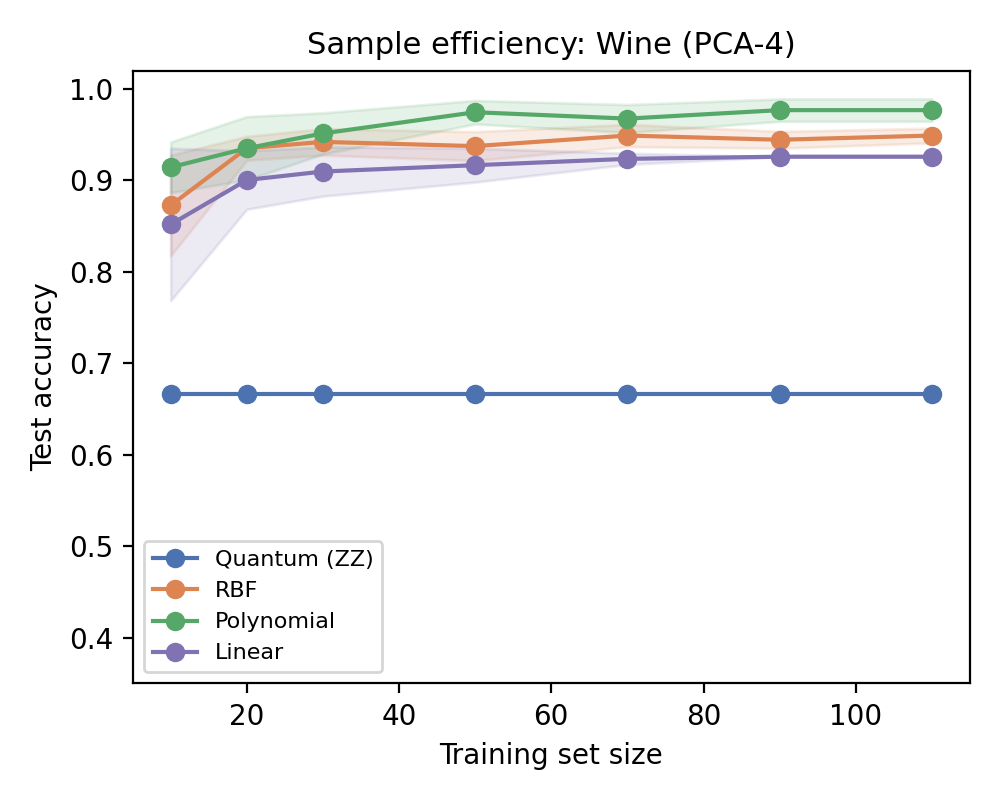
\includegraphics[width=\textwidth]{../figures/learning_curve_wine.png}
  \end{subfigure}
  \caption{Test accuracy vs.\ training set size (mean $\pm$ std over $8$
  random training subsets at each size, fixed hyperparameters from
  Table~\ref{tab:main}). \textbf{Left:} engineered quantum-advantage data --
  the quantum kernel is the only one that learns. \textbf{Right:} Wine
  (real data) -- the quantum kernel is flat at the majority-class baseline
  regardless of training set size, while classical kernels learn quickly.}
  \label{fig:learning-curves}
\end{figure}

\textbf{Decision boundaries.} To visualize \emph{why} the quantum kernel
wins on engineered data, Figure~\ref{fig:boundary} shows decision regions
for a $2$-qubit version of the engineered dataset (chosen only so the
input space is plottable in 2D), together with the resulting test accuracy
for each kernel. The quantum kernel reaches $100\%$ test accuracy with a
highly fragmented decision region: the true boundary, induced by a fixed
observable measured in a randomly rotated basis, is genuinely intricate when
drawn in raw $(x_1,x_2)$ coordinates, even though it corresponds to a
single hyperplane cut in the kernel's native feature space. The RBF kernel
partially approximates this intricate region locally ($85\%$), while the
polynomial and linear kernels, which can only express comparatively smooth,
low-order boundaries, are close to chance ($52\%$, $54\%$).

\begin{figure}[t]
  \centering
  
\includegraphics[width=\textwidth]{../figures/decision_boundary.png}
  \caption{Decision regions for each kernel on a $2$-qubit engineered
  dataset (points colored by true label). Only the quantum kernel, whose
  feature space matches how the labels were generated, resolves the
  intricate true boundary exactly; classical kernels with smoother inductive
  biases cannot.}
  \label{fig:boundary}
\end{figure}

\section{Discussion}
\label{sec:discussion}

\textbf{Alignment tracks accuracy, but only within a kernel family.} Within
the classical kernels on real data, alignment and test accuracy move
together in a rough but not perfectly monotonic way (e.g.\ on Breast Cancer,
alignment increases from $0.10$ to $0.29$ as RBF's $\gamma$ grows, while
accuracy peaks in the middle of that range before a mild overfitting-driven
drop) -- consistent with alignment being a useful, if imperfect, proxy for
kernel quality \citep{cristianini2001kernel}. But alignment values alone do
not explain the quantum-vs-classical gap in Table~\ref{tab:main}: the
quantum kernel's alignment on Wine ($0.108$) is comparable to, or even
higher than, several classical settings with far higher accuracy, and higher
than its own alignment on the engineered $n{=}6$ dataset ($0.095$) where it
nonetheless generalizes far better. Alignment computed on the training fold
captures how separable the \emph{training} labels look under the kernel, but
does not on its own diagnose whether that separability will transfer to
unseen points, particularly for a kernel whose off-diagonal values are
weak and diffuse to begin with.

\textbf{Kernel concentration, not just alignment.} A direct check of the raw
kernel values is more revealing. Off-diagonal quantum-kernel entries on Wine
have mean $0.081$ and standard deviation $0.077$; on the engineered $n{=}4$
dataset the corresponding statistics are $0.069$ and $0.068$ -- nearly
identical, and both close to $1/2^n = 1/16 = 0.0625$, the value expected for
Haar-random states. In other words, the quantum kernel is similarly
``concentrated'' -- most points look almost equally (dis)similar to each
other -- on \emph{both} datasets; concentration alone, as studied by
\citet{thanasilp2024exponential}, does not distinguish the case where the
kernel works from the case where it does not. What differs is whether the
few non-negligible off-diagonal similarities that do survive line up with
the actual labels. On the engineered dataset they do, by construction: the
labeling rule $y(x) = \mathrm{sign}\langle\phi(x)|M|\phi(x)\rangle$ is
defined directly from the same feature map that the kernel measures
similarity in, so the SVM's max-margin hyperplane in that induced space is,
by design, close to the true decision rule. On Wine, the labels have no
relationship whatsoever to the randomly chosen $V$ and observable mask that
would have to align with them, so the concentrated, largely unstructured
similarities give the SVM nothing to exploit and it falls back to the
majority-class solution -- precisely the failure mode
\citet{thanasilp2024exponential} predict, and an instance of the general
inductive-bias mismatch formalized by \citet{kubler2021inductive}: a
generic quantum feature map is only a good prior for tasks whose structure
happens to match it, and there is no reason a priori for Wine or Breast
Cancer classification to have that structure.

\textbf{Limitations.} (1) Exact simulation restricts us to $n \le 6$ qubits;
we make no claim about behavior at the qubit counts where a quantum
computer would offer a computational advantage, nor about runtime -- our
claim is purely about statistical generalization at accessible scale. (2)
We test one feature map (ZZ, full entanglement, $R{=}2$) and two real
datasets; other feature maps (e.g.\ data re-uploading or trainable
ansätze) or a wider benchmark suite could behave differently, and a larger
study is needed before drawing conclusions about quantum kernels in
general rather than this specific, widely-used construction. (3) Our
PCA-to-4-dimensions preprocessing, chosen to match a small qubit count, may
itself discard information a classical kernel operating on the full feature
set could have used; we control for this by feeding classical kernels the
same reduced representation, but a practitioner would not normally handicap
a classical baseline this way. (4) We select $C$ (and, for classical
kernels, one additional kernel hyperparameter) by cross-validation, but do
not tune the quantum feature map's own hyperparameters (number of qubits,
repetitions, entanglement pattern) as extensively as we tune the classical
kernels' hyperparameters, since the ZZ feature map has no natural analogue
of $\gamma$ or degree beyond $R$; a more exhaustive search over feature-map
variants is left to future work.

\textbf{Broader impact.} This is a small-scale, fully classical simulation
study with no direct societal impact; we note it mainly as a caution
against over-claiming quantum advantage in applied machine learning
settings on the basis of feature-space size alone, and as a worked example
that a claimed advantage should be checked against simple, well-tuned
classical baselines under matched protocols before being reported.

\section{Conclusion}

Using a from-scratch, validated, exact simulation of the ZZ feature-map
quantum kernel, we show that whether this kernel helps or hurts is entirely
a function of whether the data's structure matches the feature map, not an
intrinsic property of ``being quantum.'' On data engineered to match it, the
quantum kernel dominates classical baselines by up to $50$ points of test
accuracy and is the only kernel that benefits from additional training
data; on unmodified real tabular data, it collapses to the majority-class
baseline while classical kernels reach $92$--$98\%$ accuracy under an
identical protocol. This gap is explained by a combination of concentrated
off-diagonal kernel values and, critically, the absence of any relationship
between those values and the real labels -- consistent with existing
inductive-bias and concentration theory for quantum kernels. We release our
simulator, datasets, and evaluation code so this protocol can be extended to
other feature maps and benchmarks.

\bibliographystyle{plainnat}
\bibliography{references}

\end{document}
